%% ============================================================
%% main.tex -- metadata, abstract, contributions, and section arc
%% Build: latexmk -pdf main.tex
%% ============================================================
\documentclass[10pt]{article}

%% ============================================================
%% style.tex -- visual and structural system
%% The baseline follows raw/processed/ZOOK.pdf:
%% letter paper, Latin Modern, one column, restrained hierarchy.
%% ============================================================

\usepackage[T1]{fontenc}
\usepackage{lmodern}
\usepackage{microtype}
\usepackage[letterpaper,margin=1in,footskip=0.45in]{geometry}

\usepackage{amsmath,amssymb,amsthm}
\usepackage{aliascnt}
\usepackage{array}
\usepackage{booktabs}
\usepackage{tabularx}
\usepackage{graphicx}
\usepackage{float}
\usepackage{xcolor}
\usepackage{xspace}
\usepackage{enumitem}
\usepackage{needspace}
\usepackage{caption}
\usepackage[colorlinks=true]{hyperref}
\usepackage[capitalize,noabbrev]{cleveref}

%% Quiet page, as in the reference paper.
\pagestyle{plain}
\setcounter{secnumdepth}{2}
\setcounter{tocdepth}{2}
\setlength{\parindent}{1.5em}
\setlength{\parskip}{0pt}
\setlength{\emergencystretch}{2em}
\setlist{nosep,leftmargin=1.5em}

%% Let large floats (the evidence register, the cost figure) share a page with
%% body text rather than being pushed onto a float-only page.
\renewcommand{\topfraction}{0.92}
\renewcommand{\bottomfraction}{0.85}
\renewcommand{\textfraction}{0.06}
\renewcommand{\floatpagefraction}{0.6}
\setcounter{topnumber}{3}
\setcounter{bottomnumber}{2}
\setcounter{totalnumber}{5}
%% Tighten the whitespace around floats so a figure and table can share a dense
%% page without forcing body text onto a new one.
\setlength{\textfloatsep}{8pt plus 2pt minus 2pt}
\setlength{\floatsep}{8pt plus 2pt minus 2pt}
\setlength{\intextsep}{8pt plus 2pt minus 2pt}

%% Semantic palette: pale sage-green family.
%% Tint #E2EEE0 (pale sage / mist green) anchors the callout background;
%% the deep and mid accents are drawn from the same eucalyptus family.
\definecolor{reportsage}{HTML}{344E41}      % deep eucalyptus: text, links, headings
\definecolor{reportsagemid}{HTML}{588157}   % mid sage: urls
\definecolor{reportsagetint}{HTML}{E2EEE0}  % pale sage: callout background
%% Backwards-compatible aliases: names retained, colours now sage green.
\colorlet{reportblue}{reportsage}
\colorlet{reportbluemid}{reportsagemid}
\colorlet{reportbluetint}{reportsagetint}
\definecolor{reportgrey}{HTML}{6B6B6B}
\definecolor{reportrule}{HTML}{D9E1EA}

\hypersetup{
  pdftitle={Short Report},
  colorlinks=true,
  linkcolor=reportblue,
  citecolor=reportblue,
  urlcolor=reportbluemid
}

%% Captions remain close to the reference's serif texture.
\captionsetup{
  font=small,
  labelfont=bf,
  justification=raggedright,
  singlelinecheck=false
}

%% ZOOK-like theorem texture: bold label, italic finding.
\newtheoremstyle{reportplain}
  {0.75\baselineskip}{0.55\baselineskip}
  {\itshape}{}{\bfseries}{.}{0.5em}{}
\newtheoremstyle{reportdefinition}
  {0.75\baselineskip}{0.55\baselineskip}
  {\normalfont}{}{\bfseries}{.}{0.5em}{}
%% All theorem-like environments share the `finding' counter so they number
%% continuously per section (3.1, 3.2, ...).  We tie them with aliascnt rather
%% than \newtheorem's optional argument: a plain shared counter makes cleveref
%% label every cross-reference "Finding", whereas aliascnt keeps the shared
%% numbering while letting cleveref name each type correctly.
\theoremstyle{reportplain}
\newtheorem{finding}{Finding}[section]
\newaliascnt{proposition}{finding}
\newtheorem{proposition}[proposition]{Proposition}
\aliascntresetthe{proposition}
\theoremstyle{reportdefinition}
\newaliascnt{definition}{finding}
\newtheorem{definition}[definition]{Definition}
\aliascntresetthe{definition}
\newaliascnt{experiment}{finding}
\newtheorem{experiment}[experiment]{Experiment}
\aliascntresetthe{experiment}
\newaliascnt{method}{finding}
\newtheorem{method}[method]{Method}
\aliascntresetthe{method}
\newaliascnt{limitation}{finding}
\newtheorem{limitation}[limitation]{Limitation}
\aliascntresetthe{limitation}

\crefname{finding}{Finding}{Findings}
\crefname{proposition}{Proposition}{Propositions}
\crefname{definition}{Definition}{Definitions}
\crefname{experiment}{Experiment}{Experiments}
\crefname{method}{Method}{Methods}
\crefname{limitation}{Limitation}{Limitations}

%% Metadata-only title system. Keep title geometry out of main.tex.
\newcommand{\reporttitle}[1]{\def\thereporttitle{#1}}
\newcommand{\reportsubtitle}[1]{\def\thereportsubtitle{#1}}
\newcommand{\reportauthors}[1]{\def\thereportauthors{#1}}
\newcommand{\reportdate}[1]{\def\thereportdate{#1}}
\reporttitle{Untitled Report}
\reportsubtitle{}
\reportauthors{Anonymous}
\reportdate{\today}

\newcommand{\makereporttitle}{%
  \begin{center}
    \vspace*{1.3em}
    {\LARGE \thereporttitle\par}
    \ifx\thereportsubtitle\empty\else
      \vspace{0.55em}{\large\itshape \thereportsubtitle\par}
    \fi
    \vspace{2em}
    {\large \thereportauthors\par}
    \vspace{1.25em}
    {\large \thereportdate\par}
  \end{center}
  \vspace{1.25em}
}

%% One presentation-like callout per report, usually after the abstract
%% or at the start of Results. It deliberately avoids rounded cards.
\newcommand{\resultcard}[2]{%
  \par\medskip
  \begingroup
  \setlength{\fboxsep}{8pt}%
  \noindent\colorbox{reportbluetint}{%
    \parbox{\dimexpr\linewidth-2\fboxsep\relax}{%
      \textbf{\color{reportblue}#1.} \color{black}#2%
    }%
  }%
  \endgroup
  \par\medskip
}

%% Plain framed box for a statement the rest of the report instantiates.
%% Deliberately unstyled: a thin rule, no tint, no card geometry.
\newsavebox{\ruleboxcontent}
\newenvironment{rulebox}{%
  \par\medskip
  \setlength{\fboxsep}{10pt}%
  \setlength{\fboxrule}{0.6pt}%
  \begin{lrbox}{\ruleboxcontent}%
  \begin{minipage}{\dimexpr\linewidth-2\fboxsep-2\fboxrule\relax}%
}{%
  \end{minipage}%
  \end{lrbox}%
  \noindent\fbox{\usebox{\ruleboxcontent}}%
  \par\medskip
}

\newcommand{\takeaway}[1]{%
  \par\smallskip\noindent\textbf{Takeaway.} #1\par
}

\newcommand{\sectionclaim}[1]{%
  \par\noindent{\color{reportblue}\textbf{#1}}\par\smallskip
}

\newcommand{\reportsection}[1]{%
  \Needspace{8\baselineskip}%
  \section{#1}%
}

\newcommand{\reportkeywords}[1]{%
  \par\smallskip\noindent\textbf{Keywords:} #1\par
}

%% ============================================================
%% macros.tex -- notation and editorial semantics
%% ============================================================

\newcommand{\ie}{\emph{i.e.}\xspace}
\newcommand{\eg}{\emph{e.g.}\xspace}
\newcommand{\cf}{\emph{cf.}\xspace}
\newcommand{\etal}{et al.\xspace}
\newcommand{\wrt}{w.r.t.\xspace}

\newcommand{\ours}[1]{\textcolor{reportblue}{#1}}
\newcommand{\baseline}[1]{\textcolor{reportgrey}{#1}}
\newcommand{\status}[1]{%
  {\footnotesize\textsf{\textcolor{reportgrey}{[\,#1\,]}}}\xspace
}

%% Algorithms.
\newcommand{\algo}[1]{\ensuremath{\mathsf{#1}}}
\newcommand{\Setup}{\algo{Setup}}
\newcommand{\Gen}{\algo{Gen}}
\newcommand{\Commit}{\algo{Commit}}
\newcommand{\Open}{\algo{Open}}
\newcommand{\Verify}{\algo{Verify}}
\newcommand{\VCCheck}{\algo{Check}}
\newcommand{\CacheExtract}{\algo{CacheExtract}}

%% Scheme and spaces.
\newcommand{\VC}{\ensuremath{\mathsf{VC}}}
\newcommand{\MT}{\ensuremath{\mathsf{MT}}}
\newcommand{\MTSymbol}{\ensuremath{\mathsf{MT}}}
\newcommand{\MTConstructor}[4]{\ensuremath{\mathsf{MT}[#1,#2,#3,#4]}}
\newcommand{\MTCommit}{\ensuremath{\mathsf{MT}.\mathsf{Commit}}}
\newcommand{\MTOpen}{\ensuremath{\mathsf{MT}.\mathsf{Open}}}
\newcommand{\MTCheck}{\ensuremath{\mathsf{MT}.\mathsf{Check}}}
\newcommand{\MTAlphabet}{\ensuremath{\Sigma}}
\newcommand{\MTMessageLength}{\ensuremath{\ell}}
\newcommand{\MTSaltSize}{\ensuremath{s}}
\newcommand{\MTMessageVector}{\ensuremath{\mathbf{m}}}
\newcommand{\MTMessageIndexSet}{\ensuremath{I}}
\newcommand{\MTMessageSubVector}{\ensuremath{\mathbf{a}}}
\newcommand{\MTCommitment}{\ensuremath{\mathsf{rt}}}
\newcommand{\MTTrapdoor}{\ensuremath{\mathsf{td}}}
\newcommand{\MTProof}{\ensuremath{\mathsf{pf}}}
\newcommand{\ROOutputSize}{\ensuremath{\sigma}}
\newcommand{\ROFunction}{\ensuremath{f}}
\newcommand{\RODistribution}[1]{\ensuremath{\mathcal{U}_{\scriptscriptstyle\mathrm{b}}(#1)}}
\newcommand{\msgspace}{\ensuremath{\mathcal{M}}}
\newcommand{\idxspace}{\ensuremath{\mathcal{K}}}
\newcommand{\commspace}{\ensuremath{\mathcal{C}}}
\newcommand{\proofspace}{\ensuremath{\Pi}}
\newcommand{\rndspace}{\ensuremath{\mathcal{R}}}
\newcommand{\bits}{\ensuremath{\{0,1\}}}
\newcommand{\N}{\ensuremath{\mathbb{N}}}
\newcommand{\field}{\ensuremath{\mathbb{F}}}

%% Objects and parameters.
\newcommand{\secpar}{\ensuremath{\lambda}}
\newcommand{\digestbits}{\ensuremath{\kappa}}
\newcommand{\saltbits}{\ensuremath{s}}
\newcommand{\msglen}{\ensuremath{\ell}}
\newcommand{\openbudget}{\ensuremath{Q}}
\newcommand{\querybudget}{\ensuremath{q}}
\newcommand{\shape}{\ensuremath{\mathsf{shape}}}
\newcommand{\vk}{\ensuremath{\mathsf{vk}}}
\newcommand{\querybits}{\ensuremath{h}}
\newcommand{\ThetaVC}{\ensuremath{\Theta}}
\newcommand{\msgvec}{\ensuremath{\mathbf{m}}}
\newcommand{\comm}{\ensuremath{\mathsf{cm}}}
\newcommand{\aux}{\ensuremath{\mathsf{aux}}}
\newcommand{\opening}{\ensuremath{\mathsf{pf}}}
\newcommand{\pp}{\ensuremath{\mathsf{pp}}}
\newcommand{\td}{\ensuremath{\mathsf{td}}}
\newcommand{\idxset}{\ensuremath{I}}
\newcommand{\RO}{\ensuremath{H}}
\newcommand{\adv}{\ensuremath{\mathcal{A}}}
\newcommand{\ext}{\ensuremath{\mathcal{E}}}
\newcommand{\Exp}[1]{\ensuremath{\mathsf{Exp}^{\RO}_{#1}}}
\newcommand{\Adv}[1]{\ensuremath{\mathsf{Adv}^{#1}_{\VC,\adv}}}
\newcommand{\sample}{\ensuremath{\stackrel{\$}{\leftarrow}}}
\newcommand{\negl}{\ensuremath{\mathsf{negl}(\secpar)}}

%% Lean-facing names.
\newcommand{\code}[1]{\texttt{#1}}
\newcommand{\collisionBound}{\ensuremath{\mathsf{collisionBound}}}
\newcommand{\MeetsBindingTarget}{\ensuremath{\mathsf{MeetsBindingTarget}}}


\reporttitle{Merkle Commitments for \textsf{Arkworks}}
\reportauthors{%
  \begin{tabular}{c@{\hspace{3em}}c}
    Alexander J. Havlin & Andrew Zitek-Estrada \\
    \texttt{alexander.havlin@epfl.ch} & \texttt{andrew.zitek@epfl.ch} \\
    EPFL & EPFL
  \end{tabular}
}
\reportdate{June 2026}

\begin{document}

\makereporttitle

\begin{abstract}
Merkle commitments are the hash-based vector commitments that post-quantum
proving systems are compiled through, so an argument inherits its soundness and
zero knowledge directly from the commitment layer beneath it.  A correct
configuration is subtle: binding and hiding each force a parameter, a digest
width and a per-leaf salt cardinality respectively, and both move with the
field and cannot be reused unchanged across fields.  The defaults shipped with
\textsf{Arkworks}'
\textsf{ark-mt} miss this for small fields, leaving both the digest and the salt
near $30$ bits against a $\secpar=128$ target and breaking binding and hiding at
once; we demonstrate the binding break with a deliberate collision found in
$44$~seconds.  Sizing these parameters should be the infrastructure's obligation, not the
user's: \textsf{ark-vc} fixes the interface between the security definitions and
interchangeable hash implementations, and a single rule maps a configuration
$(\field,\secpar,\RO,\text{interface})$, together with a declared adversary
query budget, to the digest width and salt cardinality it must meet (or, from
concrete parameters, back to the security level they actually achieve), so an
undersized choice is \emph{detected and refused} rather than shipped.  We provide a few secure example hashers, but the
design exists so that a developer can supply their own hash and receive the
parameters that make it secure.  The report treats binding and hiding in turn,
unifies their sizing under that rule, and measures its cost, with the binding
analysis additionally carrying a machine-checked Lean~4 backing.
\end{abstract}

% \reportkeywords{vector commitments; Merkle trees; random oracle model; Lean~4;
%   binding; hiding; \textsf{ark-vc}}

\reportsection{Contributions}
\label{sec:contributions}

Merkle commitments are essential to modern proof systems, but developers often have to balance
performant systems with evolving security requirements and configurability, leaving underconfigured
schemes vulnerable. We aim to lift that burden into infrastructure.

\begin{itemize}[itemsep=0.35\baselineskip, topsep=0.35\baselineskip]
  \item \textbf{Main contribution}: we provide a rule for evaluating a Merkle commitment
  scheme's binding and hiding security against a target security parameter $\lambda$,
  field $\mathbb{F}$, hash function (or random oracle) $\mathcal{H}$, and hasher
  implementation (\cref{sec:background}).
  \item \textbf{Cost measurement}: we benchmark prover time, verifier time, and proof
  size across parameter combinations spanning three fields and two hash families,
  comparing desired security thresholds with their cost.
  \item \textbf{Machine checking our results}: we give the binding derivation formalised
  in Lean~4~\cite{ZLeanVC26}.
  \item \textbf{Batch opening consolidation}: we consolidate Arkworks' batch opening onto
  CoSet pruning, carrying forward the first semester's proof-size win over its
  prefix-pruning predecessor: roughly $360$\,kB down to roughly $33$\,kB at $4{,}096$
  opened leaves.
\end{itemize}

In two semesters of work we investigated the structure of Merkle trees and Merkle
commitments in depth, and what does and does not work in our favour.  Chronologically,
we started by looking at feature requests against the Merkle tree
implementation in Arkworks' \textit{crypto\_primitives}, which already sketched out many
missing features, evidenced by an RFC (\cref{app:rfc}).  We scoped
the problem to optimal batched index-proof pruning.  As a reference we used Chiesa and Yogev's
\emph{Building Cryptographic Proofs from Hash Functions}~\cite{CY26}, for its close
agreement with our definitions and the rigour of its proofs.  For batch proofs, the book
outlines a pruning algorithm we call \emph{CoSet pruning} (\cref{app:coset}).  Arkworks'
\textit{crypto\_primitives} used a distinct algorithm for the same objective, which we
call \emph{prefix pruning} (\cref{app:prefix}).  That comparison found no statistically
significant trade-off on prover or verifier time and significantly saved on proof size.

In the second semester we shifted to the proposed Arkworks design shift, aimed at
unifying tools that had previously been specific to individual constraint systems into
one IOR/polynomial IOP compiler (\cref{app:compilation}).  Our contribution there was scoped
to evaluating Vector Commitments and their Merkle-commitment subset for the hiding and
binding security they bring to the library.  A VC scheme must satisfy $\lambda$-bit
binding (\cref{sec:background}) and, optionally, $\lambda$-bit hiding
(\cref{sec:background}).  For a Merkle scheme, both properties are enforced through the
underlying hasher, and an undersized hasher still compiles and passes every functional
test, which is what makes the problem easy to miss.  Our research surfaced concerns that
the design shift had overlooked, and this report makes them explicit for developers and
users constructing a hasher for a target hiding and binding security level.

\reportsection{Background}
\label{sec:background}

Traditionally, when we think of Merkle trees we think of arity $2$ throughout, one hasher
$f$ at every level, and a simple binding claim tied to the root commitment.  As protocols
mature and the area is studied more deeply, the picture has broadened to varying arity,
mixing hashers across levels, and different flavours of binding, each motivated by
performance and recursion-friendliness. That shift complicates security analysis, and it
is easy to lose track of details that a fixed arity-$2$, single-hasher tree used to
settle by construction.

\begin{definition}[Vector commitment scheme]\label{def:vcgeneral}
A \emph{vector commitment scheme}~\cite{CF13} over alphabet $\MTAlphabet$ and length
$\MTMessageLength$ is a triple $\VC=(\Commit,\Open,\VCCheck)$:
\begin{itemize}
  \item $\Commit(\msgvec)\to(\comm,\aux)$ binds a message
  $\msgvec\in\MTAlphabet^{\MTMessageLength}$ to a short commitment $\comm$ and
  retains a state $\aux$;
  \item $\Open(\aux,\idxset)\to\opening$ authenticates an index set
  $\idxset\subseteq[\MTMessageLength]$;
  \item $\VCCheck(\comm,\idxset,\MTMessageSubVector,\opening)\to\bits$ decides
  whether $\opening$ authenticates the subvector $\MTMessageSubVector$ at
  $\idxset$ against $\comm$, where for an honest committer
  $\MTMessageSubVector$ is exactly the committed message $\msgvec$ restricted
  to the positions in $\idxset$.
\end{itemize}
A scheme is \emph{complete} (\cref{def:vc-complete}) and \emph{position-binding}
(\cref{def:vc-binding}).  It may also implement optional extensions, namely hiding
(\cref{def:vc-hiding}), updatability, aggregation, functional opening, and
knowledge soundness, of which this report treats only hiding.
\end{definition}

\begin{definition}[Completeness]\label{def:vc-complete}
$\VC$ is \emph{complete} if for every $\msgvec\in\MTAlphabet^{\MTMessageLength}$
and every $\idxset\subseteq[\MTMessageLength]$ the honest
$\Commit$--$\Open$--$\VCCheck$ round trip accepts $\msgvec_{\idxset}$ with
probability~$1$.  For Merkle this is honest reconstruction of the root from an
opening.
\end{definition}

\begin{definition}[Merkle commitment scheme]
The \emph{Merkle commitment scheme}~\cite{Merkle88}
$\MTSymbol=(\MTCommit,\allowbreak\MTOpen,\allowbreak\MTCheck)$
instantiates \cref{def:vcgeneral} in the random-oracle model over a general
Merkle shape $G_\ell$ of depth $d=\max_i d_i$, the deepest of the per-leaf depths
$d_i$ over leaves $i$: the three algorithms query a
shared oracle $\ROFunction$, the commitment is the tree root, and the committer
state is the retained salts and labels.  The binary tree is the arity-$2$ subset
of this shape.  Two parameters carry the security: the digest
width $\digestbits$ governs binding and the salt size $\MTSaltSize$ governs
hiding, with no tuning of one supplying what the other lacks.
\end{definition}

Binding is required of every scheme in this report, and hiding matters only where the
protocol built on top needs zero-knowledge. At the \code{MerkleHasher} trait of
\textsf{ark-mt} the digest and salt widths are associated
types, fixed by whoever writes the implementation, and nothing compares them against the
size of the field.  BabyBear at $\secpar=128$ therefore gets a one-element digest over a
${\sim}30$-bit space and a one-element salt carrying ${\sim}30$ bits of entropy.  The
book~\cite{CY26} reaches the same figure and observes that such an instantiation is not
flawed as such, since a protocol may bound the prover's Merkle queries far below the
birthday threshold and argue security from its own soundness analysis.  The trait gives
no way to declare that bound, which is the role of $h$ in the rule below.

%% V2 copy of the design rule, boxed in Background so Binding and Hiding can
%% instantiate it without forward reference.  This box states the rule, and the
%% justification follows it in Background.

\begin{rulebox}
\noindent\textbf{The design rule.}\quad
A protocol designer supplies five things: a field~$\field$, a security
level~$\secpar$, a hash~$H$, a choice of standard or hiding interface, and an
adversary model, declared as the query-budget exponent~$h$.  Everything else
is derived.  From $(\field,\secpar,h)$ the parameter constructor produces
\begin{equation}\label{eq:rule}
  D=\left\lceil\frac{\secpar+1+2h}{b}\right\rceil,\qquad
  k=\left\lceil\frac{\secpar}{b}\right\rceil,\qquad
  S=\left\lceil\frac{\secpar}{8}\right\rceil,
\end{equation}
where $b=\lfloor\log_2|\field|\rfloor$ is the conservative bits-per-element.
Here $D$ is the digest width in field elements, and $k$, $S$ are the field-
and byte-salt cardinalities.  Each output is a checkable obligation.  The
constructor either meets it and emits the derived parameters, or it refuses.
A designer can therefore neither quietly under-specify nor silently
over-claim.
\end{rulebox}


The justification is short.  A $\querybudget\le2^{h}$-query collision search succeeds
against a $\digestbits$-bit digest with probability about
$\querybudget^2/2^{\digestbits+1}$, so meeting $2^{-\secpar}$ needs
$\digestbits\ge\secpar+1+2h$ bits, and $D$ is that floor in field elements
(\cref{lem:birthday}).  The salt is attacked one guess at a time, so $k$ and $S$ give it
$\secpar$ bits of entropy in the hash's native unit.

The query budget is where the adversary model enters, and it is the one input the
constructor cannot derive: a prover that grinds a Fiat--Shamir transcript spends its whole
query budget searching for a favourable challenge, which is why the designer declares $h$
rather than the constructor inferring it.

The report follows the rule by property from here.  \Cref{sec:binding} and
\cref{sec:hiding} each carry their own definition, failure, and derived parameter, and
\cref{sec:cost} measures what the derived parameters cost to run.

\reportsection{Binding}
\label{sec:binding}
Binding is a key property of any vector commitment scheme, and different schemes have
different notions of it~\cite{CY26}: subvector position binding, its single-position
specialisation, and the weak variant that requires an honestly generated commitment. We
look at subvector position binding of a Merkle commitment scheme and show that it can be
reduced to the collision resistance of the underlying hash function. For a given hash
function, collision resistance gives us a bound that we can evaluate against the desired
security parameter. Specifically, we show that this bound falls short of common target
$\lambda$-bit collision resistance for single field elements in small fields. The size of
the digest output by a concrete hasher is inextricably linked to the underlying field we
operate over. This realisation led us to flag a bug in Arkworks in which the hasher
implementation would output a single field element (digest size) regardless of the size of
the underlying field.

\begin{definition}[Subvector position binding]\label{def:vc-binding}
$\VC$ is \emph{subvector position binding} if no efficient adversary outputs a commitment
$\comm$ with two accepted openings
$(\idxset_b,\MTMessageSubVector_b,\opening_b)$ that disagree at some
$i\in\idxset_0\cap\idxset_1$, except with probability $\negl$.  The commitment
has no honest-generation requirement.
\end{definition}

\begin{proposition}[Binding from collision resistance]\label{thm:binding-cr}
Let $\MT[\RO]$ be a Merkle commitment over a perfect binary tree of depth $d$ whose leaf
encoding is injective and whose leaf and internal-node calls are domain separated.  If
the shared $\digestbits$-bit oracle receives at most $\querybudget$ distinct
queries during the complete experiment, then
\[
  \Adv{bind}(\ThetaVC)
  \le \Pr[\text{oracle-trace collision}]
  \le \frac{\querybudget(\querybudget-1)}{2^{\digestbits+1}},
\]
which meets $2^{-\secpar}$ when $\querybudget\le2^{h}$ and
$\secpar+1+2h\le\digestbits$.
\status{Lean-backed}
\end{proposition}

The binary tree is the case Chiesa and Yogev prove directly, and we take their proof as
given~\cite{CY26}: either the adversary's query trace already contains a collision, or the
two accepted openings of the minimal disputed index yield one across the two verification
traces, bounded by a union bound over the at most $(d+1)^2$ query pairs.  This is the
straightforward form the book states before improving on it, and the form \cref{eq:rule}
consumes.  The reduction is machine-checked in Lean~4~\cite{ZLeanVC26} for a general Merkle
shape, closed for singleton openings and argued on paper for a general index set
(\cref{app:binding-generic}).

Now that we have seen the reduction to collision resistance, consider how a hasher is
implemented concretely. Every hasher in \textsf{ark-mt} satisfies one \code{MerkleHasher}
trait (\cref{app:hasher-trait}), and the current Poseidon2 implementation sets its digest
to one field element, for every field $\mathbb{F}$ and every target $\lambda$. Nothing in
the trait or the implementation reads $\lambda$.

Now suppose we set a target security parameter $\lambda=128$. BabyBear's modulus is
$p=2013265921$, a $31$-bit prime, and the conservative bound used throughout this report is
$b=\lfloor\log_2 p\rfloor=30$ bits per element, so a one-element digest publishes a root drawn
from a $30$-bit space. Applying \Cref{lem:birthday} at $\digestbits=30$, a collision search
succeeds once the query count passes roughly $2^{15.5}\approx46{,}000$, well short of a
$\lambda=128$ target.

The book states this result plainly for a $31$-bit field. We ran
the search only to confirm that the one-element preset sits in that regime, and it produced two
trees over different messages sharing one root in $44$ seconds on a commodity laptop,
averaged over three seeded runs (\cref{app:demo}). The collision is cross-shape, between an
$8$-leaf binary tree and an $8$-leaf $8$-ary tree on the same Poseidon2 instance, and it
still breaks \Cref{def:vc-binding} as stated because \code{hash\_leaf} and
\code{hash\_nodes} carry no layer, index, or arity tag (\cref{lem:geometry}). Working
backwards from $\lambda$ and $\mathbb{F}$, \cref{eq:rule} asks for
$D=\lceil257/30\rceil=9$ elements at $\lambda=128$ and $h=64$, so fixing the hasher means
widening \code{Digest} from \code{F} to a nine-element array and hashing into all nine on
every call, which we price in \Cref{sec:cost}.
\reportsection{Hiding}
\label{sec:hiding}

A zero-knowledge protocol relies on more than hiding, and the book's stronger requirement is
\emph{equivocation}, which a Merkle commitment satisfies in the random-oracle model through
an inefficient simulator that programs the oracle, though never in the \emph{trapdoor} form
an efficient simulator would need, since there is no $\Setup$ secret to program
($\td=\bot$)~\cite{CY26}.  We work with the indistinguishability form of hiding below, which
rests entirely on the salt space, and show that the current salt is too small to carry it.

\begin{definition}[Hiding]\label{def:vc-hiding}
A randomised $\VC$ whose $\Commit$ draws salts from a space $\rndspace$ is
\emph{hiding} if, for any two messages of length $\MTMessageLength$ and any
adversary that after seeing $\comm$ adaptively opens positions on which the
messages agree, the advantage in deciding which was committed is at most
$\negl$.  For Merkle this refines to \emph{root hiding}, meaning the real root is
statistically close to one simulated without $\msgvec$, strengthened to
\emph{selective-opening hiding}, which must also hide through the disclosed
salts and authentication paths of partial openings.
\end{definition}

In a Merkle commitment scheme, we refer to salt simply as the random per-leaf nonce.
Each leaf is itself a basic commitment $H(\msgvec_i,\text{salt})$, and the salt travels
in the authentication path beside the sibling digests so the verifier can recompute
the leaf.  Opening one leaf commitment under two different salts would force a
hash collision, so the salt binds a value to its position even as it hides it.
Hiding then rests entirely on the salt space, which must be both well sampled
and large enough to resist search within the security budget, neither of which a
deterministic salt satisfies, since the receiver can recompute candidate leaf commitments.

The digest and the salt scale differently in the query budget, which is what
\cref{eq:rule} is tracking when it derives $D$ from $h$ and derives $k$ and $S$ from
$\secpar$ alone.  A binding adversary wins on any collision among its own queries, so its
advantage grows as $\querybudget^2/2^{\digestbits}$ and the digest has to carry $2h$ bits of
headroom.  A hiding adversary has to hit one particular salted leaf input, so its advantage
grows as $\msglen\querybudget/2^{\saltbits}$, and the salt needs only $\secpar$ bits.

\begin{proposition}[Salt cardinality]\label{prop:salt-card}
Let the salt be drawn from $k$ elements of a field with $b=\lfloor\log_2|\field|\rfloor$
bits per element, or from $S$ bytes.  Then $|\rndspace|\ge2^{\secpar}$ whenever
$k\ge\lceil\secpar/b\rceil$ or $S\ge\lceil\secpar/8\rceil$.
\status{Lean-backed}
\end{proposition}

This is what \cref{eq:rule} computes for $k$ and $S$ and the one part of hiding that is
machine-checked, while the bound it feeds into remains an \emph{intended reduction}
(\cref{app:hiding-reduction}).

Looking again at the Arkworks library, the current hiding hasher repeats the
undersized-parameter mistake we saw for binding, this time in the salt space
(\cref{app:hasher-trait}): the salt is one field element for every field and every target
$\lambda$, drawn uniformly, so the sampling requirement is met and what falls short is the
number of values it can take.

Take a target security parameter $\lambda=128$ and BabyBear again.  Each field element
carries at most $b=\lfloor\log_2 p\rfloor=30$ bits under the conservative accounting of
\cref{eq:rule}, so a one-element salt ranges over roughly $2^{30}$ values.  An
adversary who knows the two candidate messages recovers which was committed by hashing
$2^{30}$ candidate leaves against the opened position.  Reaching $2^{\lambda}$ instead needs
$k=\lceil\lambda/b\rceil=\lceil128/30\rceil=5$ elements.  The same constructor gives
$k=3$ for Goldilocks at $b=63$, and $k=1$ for BN254 at $b=253$, where a single element
already carries more than the target.

\reportsection{The Parametrisation Model}
\label{sec:spine}

Binding and hiding failed separately and were sized separately, but the two
sizings are one rule, and that they share a rule is the point of this section.
The earlier \textsf{Arkworks/crypto-primitives}~\cite{ArkCryptoPrimitives} bought security by hardcoding every
choice, and developers, wanting simpler hash interfaces, variable tree shapes,
and efficient multi-opening compression, asked for that freedom back.  Granting
it lets a user control $(\field,\secpar,\RO,\text{interface})$ in full, and the
danger is exactly that without hardcoded guardrails a misconfiguration stays
silent.  So the developer faces a question they cannot answer from the interface
alone: which security claim does my concrete configuration actually support?
Answering it is our obligation, not theirs.  Given those choices and a
declared adversary model, the
infrastructure owes back the parameters that must be used, a proof that they
meet the target, the cost they incur, and the property they buy.  The user can
then keep their attention on their own implementation and read its concrete
security off the guarantees we give.

\subsection{The Object It Sizes}
\label{sec:object}

We fix the commitment object once, following the Chiesa--Yogev notation so the
mathematical boundary does not drift from the reference the implementation
follows~\cite{CY26}.

\begin{definition}[Vector commitment scheme]\label{def:vcgeneral}
A \emph{vector commitment scheme}~\cite{CF13} over alphabet $\MTAlphabet$ and length
$\MTMessageLength$ is a triple $\VC=(\Commit,\Open,\VCCheck)$:
\begin{itemize}
  \item $\Commit(\msgvec)\to(\comm,\aux)$ binds a message
  $\msgvec\in\MTAlphabet^{\MTMessageLength}$ to a short commitment $\comm$ and
  retains committer state $\aux$;
  \item $\Open(\aux,\idxset)\to\opening$ authenticates an index set
  $\idxset\subseteq[\MTMessageLength]$;
  \item $\VCCheck(\comm,\idxset,\MTMessageSubVector,\opening)\to\bits$ decides
  whether $\opening$ authenticates the subvector $\MTMessageSubVector$ at
  $\idxset$ against $\comm$, where for an honest committer
  $\MTMessageSubVector$ is exactly the committed message $\msgvec$ restricted
  to the positions in $\idxset$.
\end{itemize}
A scheme is \emph{complete} (\cref{def:vc-complete}) and
\emph{position-binding} (\cref{def:vc-binding}), and may implement optional
extensions---hiding, treated here, plus updatability, aggregation, functional
opening, and knowledge soundness---which \textsf{ark-vc}'s capability model
accommodates but this report does not treat.
\end{definition}

\begin{definition}[Completeness]\label{def:vc-complete}
$\VC$ is \emph{complete} if for every $\msgvec\in\MTAlphabet^{\MTMessageLength}$
and every $\idxset\subseteq[\MTMessageLength]$ the honest
$\Commit$--$\Open$--$\VCCheck$ round trip accepts $\msgvec_{\idxset}$ with
probability~$1$.  For Merkle this is honest reconstruction of the root from an
opening.
\end{definition}

\begin{definition}[Merkle commitment scheme]\label{def:vc}
The \emph{Merkle commitment scheme}~\cite{Merkle88}
$\MTSymbol=(\MTCommit,\allowbreak\MTOpen,\allowbreak\MTCheck)$
instantiates \cref{def:vcgeneral} in the random-oracle model over a general
Merkle shape $G_\ell$ of depth $d=\max_i d_i$, the deepest of the per-leaf depths
$d_i$ over leaves $i$: the three algorithms query a
shared oracle $\ROFunction$, the commitment is the tree root, and the committer
state is the retained salts and labels.  The binary tree is the arity-$2$ subset
of this shape.  Two parameters carry the security: the digest
width $\digestbits$ governs binding and the salt size $\MTSaltSize$ governs
hiding, with no tuning of one supplying what the other lacks.
\end{definition}

\begin{limitation}[No trapdoor, so no standard-model equivocation]
\label{lim:no-trapdoor}
$\MTSymbol$ has no cryptographic $\Setup$: the public parameter is the hash
itself, so the trapdoor is empty ($\td=\bot$).  This shapes what can even be
asked of the scheme.  Extraction cannot program a trapdoor and must instead
argue from the adversary's random-oracle query trace, and standard-model
equivocation, which opens one commitment to two values precisely by
programming a trapdoor, has nothing to program.  Equivocation is therefore
unreachable for this scheme by construction, not merely unproved.
\end{limitation}

\subsection{The Rule}
\label{sec:rule}

The rule itself was stated in the box of \cref{sec:background}: from the
designer's interface-level inputs $(\field,\secpar,H,\text{interface})$ and
the declared adversary budget $h$, the constructor
derives the digest width $D$, the field-salt cardinality $k$, and the byte-salt
cardinality $S$ of \cref{eq:rule}, and either meets each obligation or refuses
the configuration.  What remains to establish here is what the rule does not
depend on, and what it produces per field.

The rule is arity-independent.  $(D,k,S)$ depends only on $(\field,\secpar,h)$,
while the tree shape and arity enter only through the query budget $h$ and the
cost.  The same target
therefore sizes any Merkle shape and produces different outputs per field: for
BabyBear ($b=30$, $h=64$) it gives $D=9$, $k=5$, $S=16$; for BN254
($b\approx254$) it gives $D=2$, $k=1$, $S=16$.  These are not interchangeable,
and the $44$-second break of \cref{sec:background} used a $D=1$ configuration,
one of the hashers \textsf{Arkworks} currently ships, which is exactly the kind
of undersizing the constructor now refuses.

\reportsection{Cost}
\label{sec:cost}

\paragraph{What the benchmarks measure.}
The rule says which configurations support a security claim, and the benchmarks say what
those configurations cost.  Each plot fixes a binary tree with $4{,}096$ leaves and $32$
openings and reports mean prover time, verifier time, and proof size.  A field-coloured
line marks the first configuration reaching $\secpar\ge128$, and a red \textsf{x} marks
each cost transition.

\paragraph{The salt arrives in the hash's native unit.}
The rule reports the salt in the hash's own unit, $k$ field elements for an algebraic hash
such as Poseidon2~\cite{GKS23}, or $S$ bytes for a byte-oriented hash such as
Blake3~\cite{BLAKE3}.  Because the unit already matches the hash, the salt pays no encoding
penalty when it is absorbed.

\paragraph{Permutations set the transitions.}
Sponge-based hash functions operate on a \textit{state} of size $t=\text{rate}+\text{capacity}$,
where the capacity carries the previous round's output and the rate is the room left to
absorb new input.  We measure how many elements a construction absorbs before it needs a
second permutation, then overlay the security the rule certifies to mark where each field
reaches the target.

%% Measured cost of the first Poseidon2 configuration reaching lambda >= 128
%% per field and per property.  Source: ark-mt security_parameters benchmark
%% (benchmark_matrix.csv); binary tree, 4,096 leaves, 32 openings.
\begin{table}[t]
  \centering
  \small
  \begin{tabular}{llrrrr}
    \toprule
    Property & Field & Parameter & Prover (ms) & Verifier (ms) & Proof (kB) \\
    \midrule
    Hiding  & BabyBear   & $k=5$ & $25.7$  & $1.03$  & $3.6$  \\
    Hiding  & Goldilocks & $k=3$ & $39.8$  & $1.51$  & $4.6$  \\
    Hiding  & BN254      & $k=1$ & $175.2$ & $6.56$  & $10.3$ \\
    \addlinespace
    Binding & BabyBear   & $D=9$ & $38.7$  & $1.84$  & $10.1$ \\
    Binding & Goldilocks & $D=5$ & $40.3$  & $1.37$  & $11.0$ \\
    Binding & BN254      & $D=2$ & $260.0$ & $11.26$ & $16.4$ \\
    \bottomrule
  \end{tabular}
  \caption{Measured cost of the first Poseidon2 configuration reaching
  $\secpar\ge128$ per field, for the hiding benchmarks (varying the salt
  cardinality $k$) and the binding benchmarks (varying the digest width $D$).
  Prover time is mean commit plus open;
  verifier time is mean check; proof size is the compressed proof.  Fixed
  regime as in \cref{fig:poseidon-cost}: binary tree, $4{,}096$ leaves, $32$
  openings.}
  \label{tab:cost-at-128}
\end{table}


\begin{figure}[t]
  \centering
  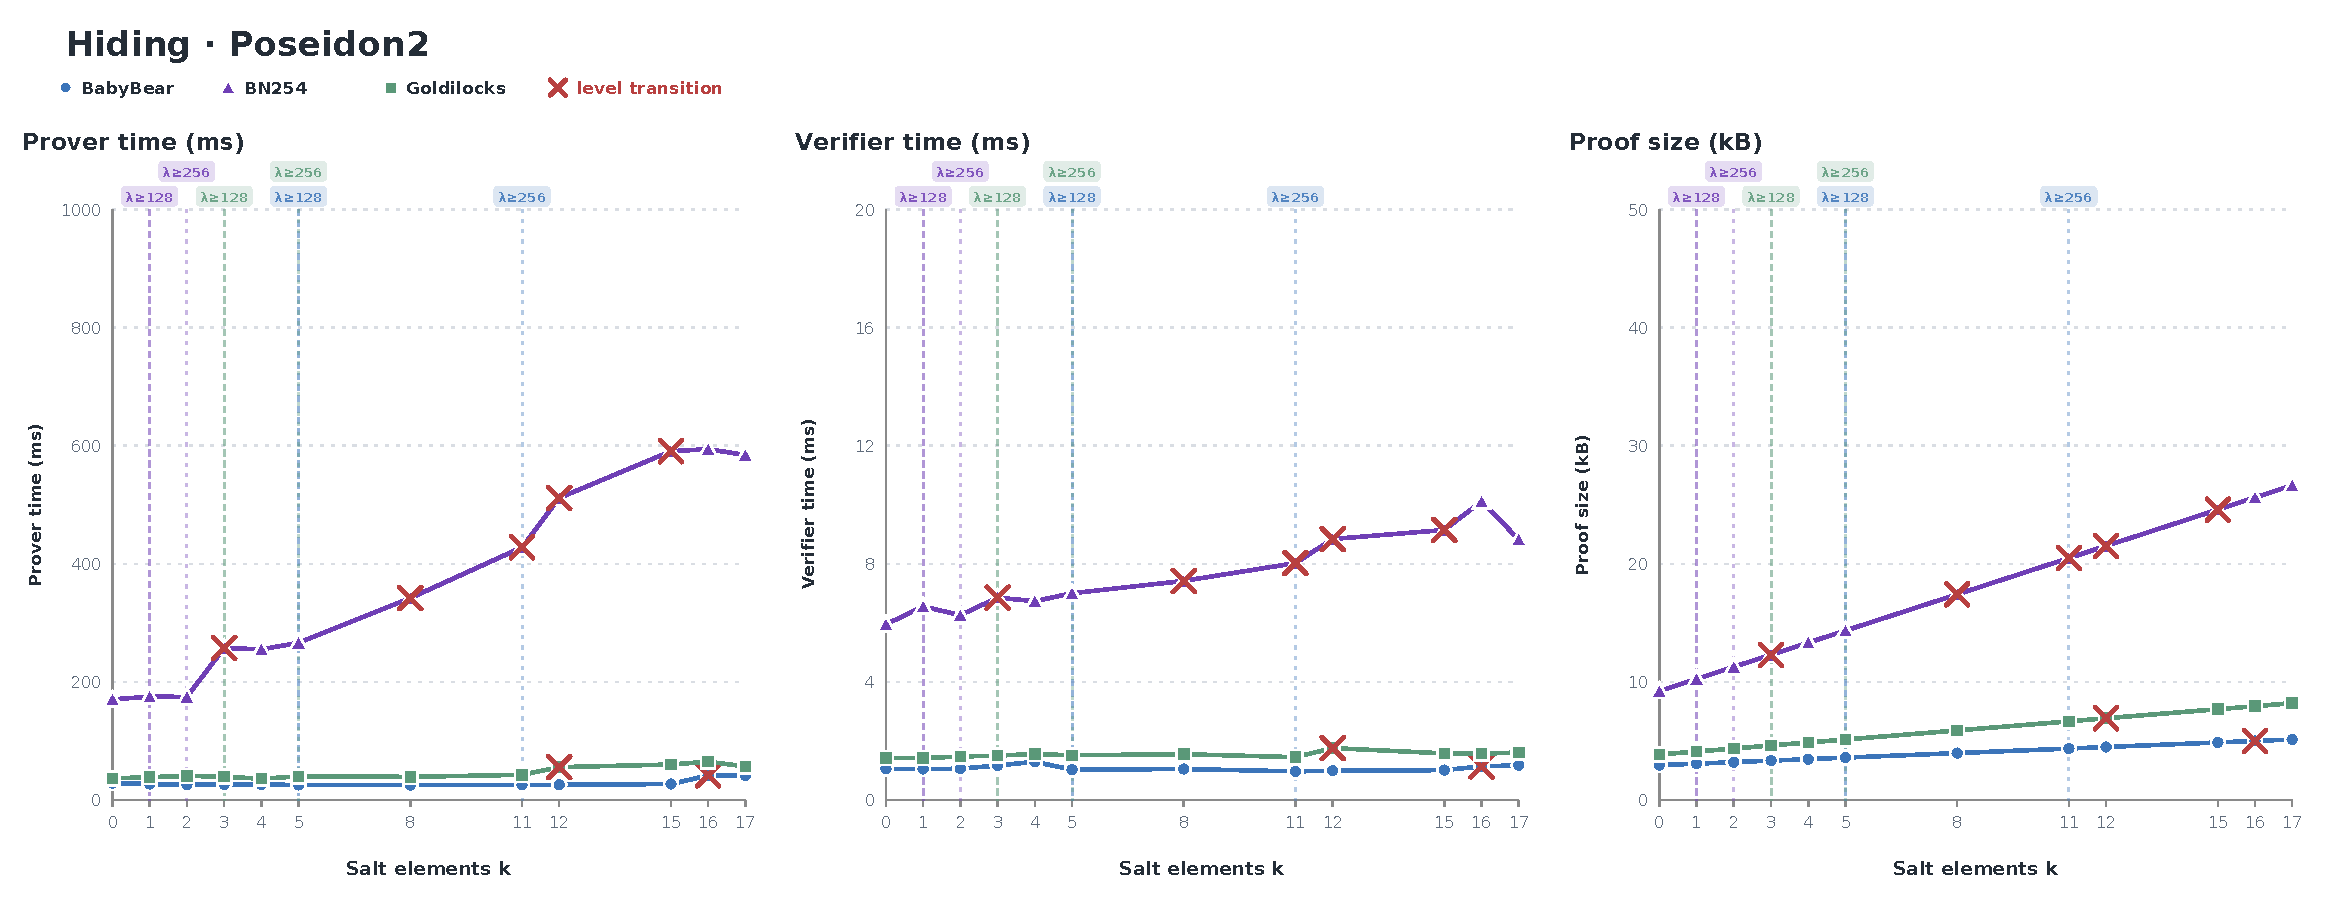
\includegraphics[width=\linewidth]{figures/benchmark_hiding_poseidon_triptych_extra_x.pdf}\\[5pt]
  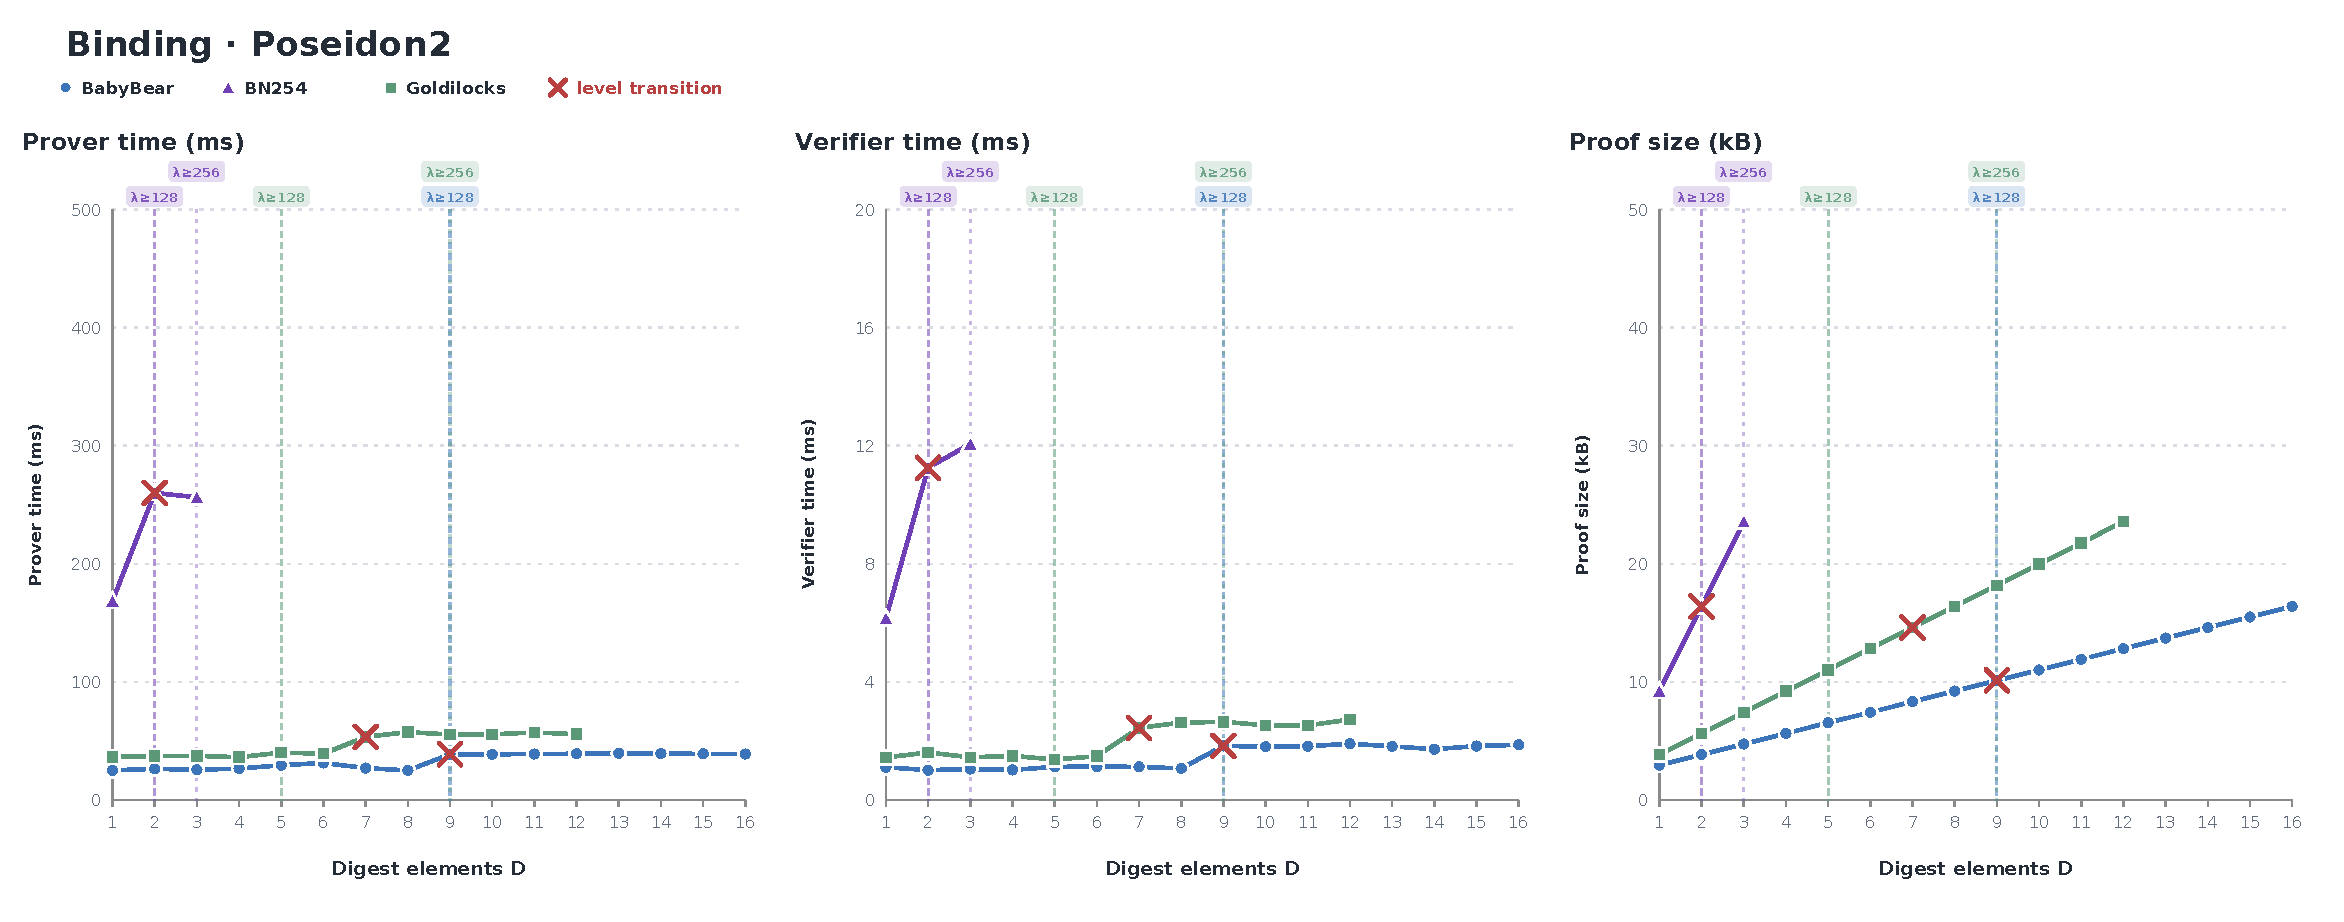
\includegraphics[width=\linewidth]{figures/benchmark_binding_poseidon_triptych_extra_x.pdf}
  \caption{Poseidon2 hiding cost as salt width grows (top) and binding cost as
  digest width grows (bottom).  Field-coloured lines mark the first measured
  $\secpar\ge128$ point for BabyBear, Goldilocks, and BN254.
  Red \textsf{x} markers flag inputs that cross into an extra permutation.}
  \label{fig:poseidon-cost}
\end{figure}

\paragraph{When binding is free.}
Proof size grows linearly with the digest width for every field, so a user with proof size
concerns can read off how much security a given size buys.  Timing has a step shape
instead: within a permutation level, widening the digest gains security at no measurable
cost, and crossing a level raises prover and verifier time sharply before flattening again.
A parent hash absorbs two child digests, so a digest is charged once per tree level while a
salt is absorbed once at the leaf, which is why a binary tree stays inside one permutation
only while $2D\le t$.  BabyBear's Poseidon2 preset runs at $t=16$ ($D\le8$ free) against a
certified $D=9$, and BN254 runs at $t=3$ ($D\le1$ free) against a certified $D=2$: both sit
one element past the boundary and pay for a second permutation, taking prover time from
$25.1$ to $38.7$~ms for BabyBear and $168.6$ to $260.0$~ms for BN254.  Goldilocks is the
exception: its $t=12$ preset holds $D\le6$ while the rule asks for only $D=5$, so its
certified binding parameters sit inside a permutation block computed anyway
(\cref{fig:hash-blocks}, left).  Proof size orders the fields the other way: Goldilocks
reaches $\secpar=128$ at fewer digest-width increments than BabyBear, yet its proof at the
crossing is the larger of the two, $11.0$ against $10.1$~kB, because each Goldilocks
element is wider.

\paragraph{Hiding is cheap everywhere.}
The rule asks for $k=5$ field salts on BabyBear, $k=3$ on Goldilocks, and $k=1$ on BN254,
while the measured leaf transitions fall at $k=16$, $k=12$, and $k=3$ respectively.  Every
field therefore reaches $\secpar=128$ well inside its first permutation block, and prover
and verifier time stay flat as the salt widens.  A user weighing hiding needs to consider
only the proof size trade-off, which grows linearly in the number of salt elements.

\paragraph{Bytewise hashers step at block boundaries.}
Blake3 compresses over fixed blocks, and an input that crosses a boundary needs a second
compression call.  Binding shows the same step structure as Poseidon2: the $\secpar=128$
digest occupies $33$ bytes, the first boundary, and crossing it takes prover time from
$1.72$ to $2.28$~ms (\cref{fig:hash-blocks}, right).  Hiding clears its own target before
the first transition, so its only cost is the proof size, which grows linearly with the
salt width.\footnote{The full bytewise Blake3 benchmark results are plotted in
\cref{fig:blake3-cost} (\cref{app:bytewise-cost}).  The prose here summarises their
result.}
\status{empirical; binary tree, $4{,}096$ leaves, $32$ openings}

\reportsection{Provenance: From Retrofit to Parametrisation Model}
\label{sec:provenance}

The first phase of this work compared the existing
\textsf{Arkworks/crypto-primitives} Merkle tree with the Chiesa--Yogev
presentation~\cite{CY26}.  It began as implementation work around open feature
requests: simplify the split hash interface, remove caller-side ordering
footguns, support richer tree shapes, and compress multi-openings.  Read
together, those requests pointed to one broader issue.  The implementation had
many locally reasonable decisions, but no single specification against which
their combined behaviour could be reviewed.

That comparison produced concrete engineering results.  The \code{CoSet}
multiproof encoding realises the book's path-pruning optimisation for
multi-openings, and \code{ImplicitCoPath} performs the same pruning without
materialising a coordinate bookkeeping layer, which is purely pedagogical when
used outside a position-tagging context.  That coordinate-encoding backing was nonetheless built out
in full, and although it sits outside this report's use, it is exactly the
groundwork the geometric, position-tagged style of binding
(\cref{sec:binding}) would build on.  The
\code{Committed}/\code{OpeningProof}/\code{Opening} split makes ordering and
duplicate-index validation part of construction rather than caller discipline.
\Cref{fig:coset-compression} shows the headline measurement: at $4{,}096$
opened leaves the clustered multiproof is roughly a tenth the size of the
per-path encoding it replaces.  The benchmark harnesses built to take that
measurement prefigure the cost benchmarks of \cref{sec:cost}.  None of this code
was merged into the current tree.

\begin{figure}[t]
  \centering
  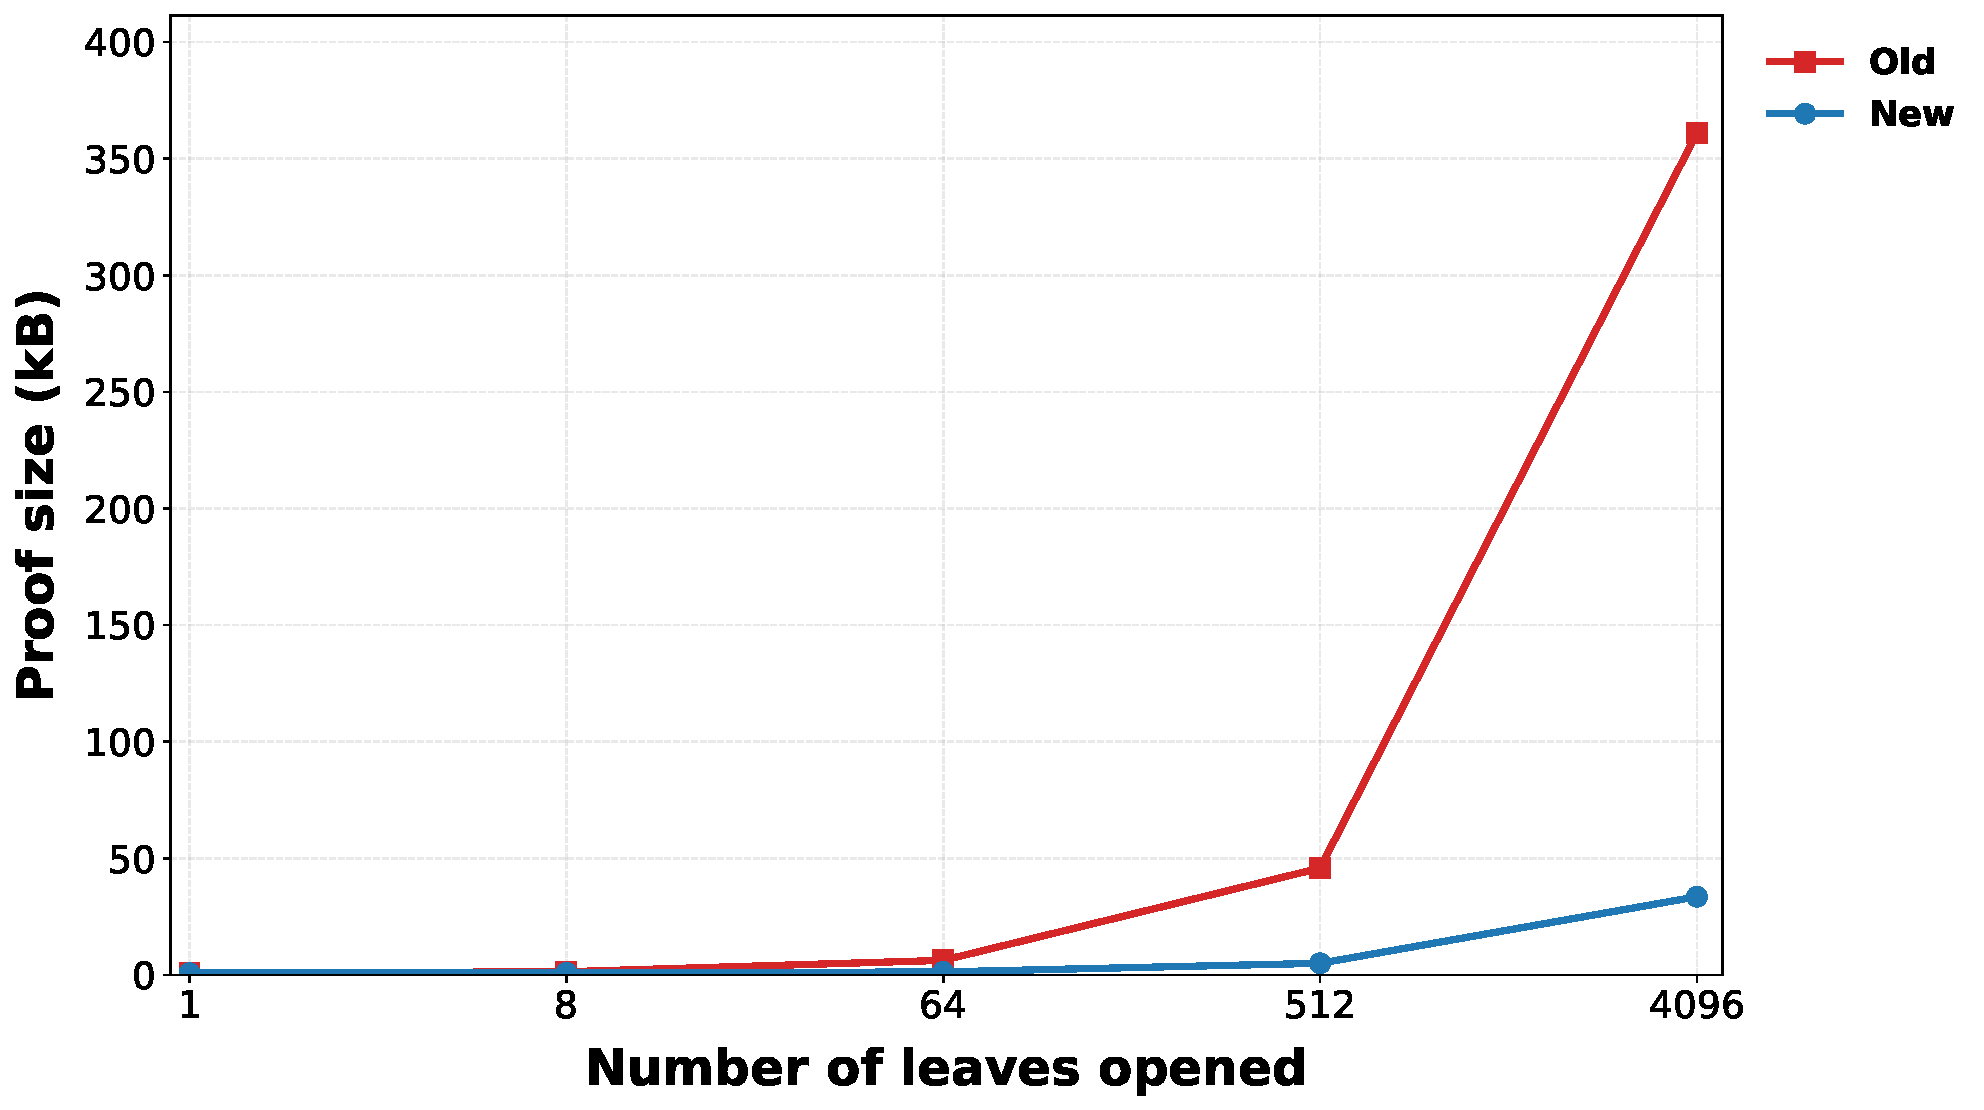
\includegraphics[width=0.5\linewidth]{figures/coset-proof-size-clustered.pdf}
  \caption{Phase-1 multiproof compression on clustered openings of a
  $4{,}096$-leaf tree.  The \code{CoSet} encoding prunes shared path material,
  so proof size grows with the disclosed frontier rather than with the number
  of individual paths: at $4{,}096$ opened leaves the compressed proof is
  roughly $33$\,kB against roughly $360$\,kB uncompressed.}
  \label{fig:coset-compression}
\end{figure}

The stronger finding was methodological.  A reference definition can organise
an API, yet an API alone still does not tell a developer which security claim a
concrete configuration supports.  That is the step from retrofit to
parametrisation model: keep the literature-facing definition, connect it to
executable interfaces, state the security games, derive the parameters, and
expose the evidence boundary.  What the semester enabled therefore runs through
the whole report.  The freedoms whose absence the retrofit exposed (simpler
hash interfaces, variable tree shapes, efficient multi-opening compression) are
exactly the ones the parametrisation model of \cref{sec:spine} grants and then
guards.  The multiproof pruning strategy survives in \textsf{ark-mt}'s capped
openings, where the commitment publishes the ordered digest layer at a chosen
depth instead of the single root, so every opening sheds that many layers of
shared copath.  The cost measurements of \cref{sec:cost} run on the
benchmarking craft built here.

\reportsection{Conclusion and Next Steps}
\label{sec:conclusion}

A vector commitment is only as strong as the parameters underneath it, and
Arkworks' current defaults miss that target for small fields on both axes at
once.  The rule of \cref{eq:rule} derives, from a designer's declared inputs,
the digest and salt parameters a security target forces, and refuses the
undersized configurations those defaults allow, including the one broken here
in $44$ seconds.  The cost benchmarks price the derived parameters and
separate the security thresholds from the cost transitions.  For Poseidon2 the
certified hiding salts fit inside permutation blocks already paid for on all
three fields, so hiding at $\secpar=128$ costs nothing extra.  Binding is free
in the same sense only on Goldilocks.  BabyBear and BN254 reach their
certified digest widths one element past the permutation boundary and pay
roughly half again in prover time for it.  That cost is what the correct
parameter is worth on those fields.  The binding reduction and the
salt-cardinality lemmas hiding needs both carry a machine-checked Lean
backing.

\paragraph{Next.}
The formal status splits three ways, and the split is the information.  Closed:
the binding chain end to end, and the salt-cardinality lemmas hiding needs.
Scoped and believed but not yet closed: the extraction bridge and one
distributional averaging step, both reduced to named deterministic pieces.
Not yet stated in the formal model: the sampling-based hiding game and
equivocation, so the hiding claim rests on the intended reduction of
\cref{sec:hiding} rather than a checked theorem.  Beyond the formalisation,
multi-round BCS and Fiat--Shamir soundness would justify the strengthened
digest target at the protocol level, and the $k$-ary and arbitrary-length
shapes share the generic binding reduction but are not yet exhibited.


\begingroup
\footnotesize
\makeatletter
\renewcommand\section{\@startsection{section}{1}{\z@}%
  {-0.8ex \@plus -0.3ex}{0.4ex}{\normalfont\large\bfseries}}
\makeatother
\bibliographystyle{alpha}
\bibliography{references}
\endgroup

\end{document}
